\chapter{Fonctions}
\introduction{Quelle est la fonction de ce chapitre ?}
\section{Exemples de fonctions}
\subsection{Un objet déjà connu}
Nous avons déjà rencontré des fonctions \textit{côté utilisateur}:
\begin{itemize}
    \item \mintinline{python}{input}
          \begin{itemize}
              \item prend en entrée une chaîne de caractères ;
              \item renvoie la chaîne de caractère saisie par l'utilisateur.
          \end{itemize}
          On peut noter ceci \mintinline{python}{input(chaine: str) -> str}
    \item \mintinline{python}{len}
          \begin{itemize}
              \item prend en entrée une liste ;
              \item renvoie le nombre d'éléments de cette liste.
          \end{itemize}
          On peut noter cela \mintinline{python}{len(lst: list) -> int}
\end{itemize}

\subsection{De multiples formes}
\floatpictureright{0.5}{img/fonction1}
{Les deux exemples précédents rentrent dans la catégorie représentée à droite.}
\medskip\par
\floatpictureleft{0.5}{img/fonction2}
{Certaines fonctions sont comme à gauche.\\
    Par exemple \mintinline{python}{max(20,3,10)} renvoie 20.}
\medskip\par
\floatpictureright{0.5}{img/fonction3}{
    D'autres fonctions sont comme à droite.\\
    On verra des exemples plus tard.}
\medskip\par
\floatpictureleft{0.5}{img/fonction4}{
    D'autres encore sont comme à gauche.\\
    Par exemple \mintinline{python}{print("salut")} ne renvoie rien mais affiche \mintinline{python}{salut} à l'écran.}
\medskip\par
\floatpictureright{0.5}{img/fonction5}{
    D'autres suivent le schéma ci-contre.\\
    Par exemple dans le module \mintinline{python}{time}, la fonction \mintinline{python}{time} ne prend aucun paramètre d'entrée mais renvoie l'heure qu'indique l'horloge de l'ordinateur.\\
    On peut par exemple l'utiliser pour stocker une heure précise en tapant \mintinline{python}{maintenant = time()}.}
\medskip\par
\floatpictureleft{0.5}{img/fonction6}{
    Enfin certaines suivent ce schéma.\\
    Par exemple dans le module \mintinline{python}{pygame}, \mintinline{python}{pygame.display.flip} ne prend aucun paramètre d'entrée, ne renvoie aucune valeur, mais actualise la fenêtre graphique.\\
    On l'appelle donc en tapant \mintinline{python}{pygame.display.flip()}.}
\medskip\par
Il est possible de créer de nouvelles fonctions.\\
On parle alors de fonctions \textit{côté concepteur}.\\

Il faut donc définir rigoureusement ce qu'est une fonction.

\section{Définition de la notion de fonction}
\begin{definition}[ : fonction]
    Une \textit{fonction} est un \og morceau de code\fg{} qui représente un \textit{sous-programme}.\\
    Elle a pour but d'effectuer une tâche \textit{de manière indépendante}.\\
\end{definition}

\begin{exemple}
    On veut modéliser la fonction mathématique $f$ définie pour tout nombre réel $x$ par $$f(x)=x^2+3x +2$$

    On écrira alors

    \begin{minted}[breaklines,breakanywhere]{python}
def f(x : float) -> float:
    return x ** 2 + 3 * x + 2
            \end{minted}

    Pour évaluer ce que vaut $f(10)$ et affecter cette valeur à une variable, on pourra désormais écrire \mintinline{python}{resultat = f(10)}.
\end{exemple}


Que fait la fonction \mintinline{python}{mystere} ?

\begin{minted}[breaklines,breakanywhere]{python}
def mystere(a : float, b : float) -> float:
    if a <= b:
        return b
    else:
        return a            
\end{minted}



La fonction \mintinline{python}{mystere}:
\begin{itemize}
    \item   prend en entrée deux paramètres de type \mintinline{python}{float} \mintinline{python}{a} et \mintinline{python}{b};
    \item   renvoie le plus grand de ces deux nombres.
\end{itemize}

La réponse que l'on vient de formuler s'appelle \textit{la spécification} de la fonction $f$.

\begin{definition}[ : fonction]
    Donner la spécification d'une fonction \mintinline{python}{f} c'est
    \begin{itemize}
        \item   préciser le(s) type(s) du (des) paramètre(s) d'entrée (s'il y en a) ;
        \item   indiquer sommairement ce que fait la fonction \mintinline{python}{f} ;
        \item   préciser le(s) type(s) de la (des) valeur(s) de sortie (s'il y en a).
    \end{itemize}
\end{definition}

\section{Anatomie d'une fonction}
\begin{pyc}
\begin{minted}{python}
def f(lst: list) -> int
    mini = lst[0]
    n = len(lst)
    for i in range(n):
        lst[i] < mini:
        mini = lst[i]
    return mini
   \end{minted}
\end{pyc}

La fonction \mintinline{python}{f}
\begin{itemize}
    \item   prend en entrée une liste (sous entendu d'entiers);
    \item   renvoie le plus petit entier de cette liste.
\end{itemize}

\subsection{Paramètre formel}
\begin{center}
    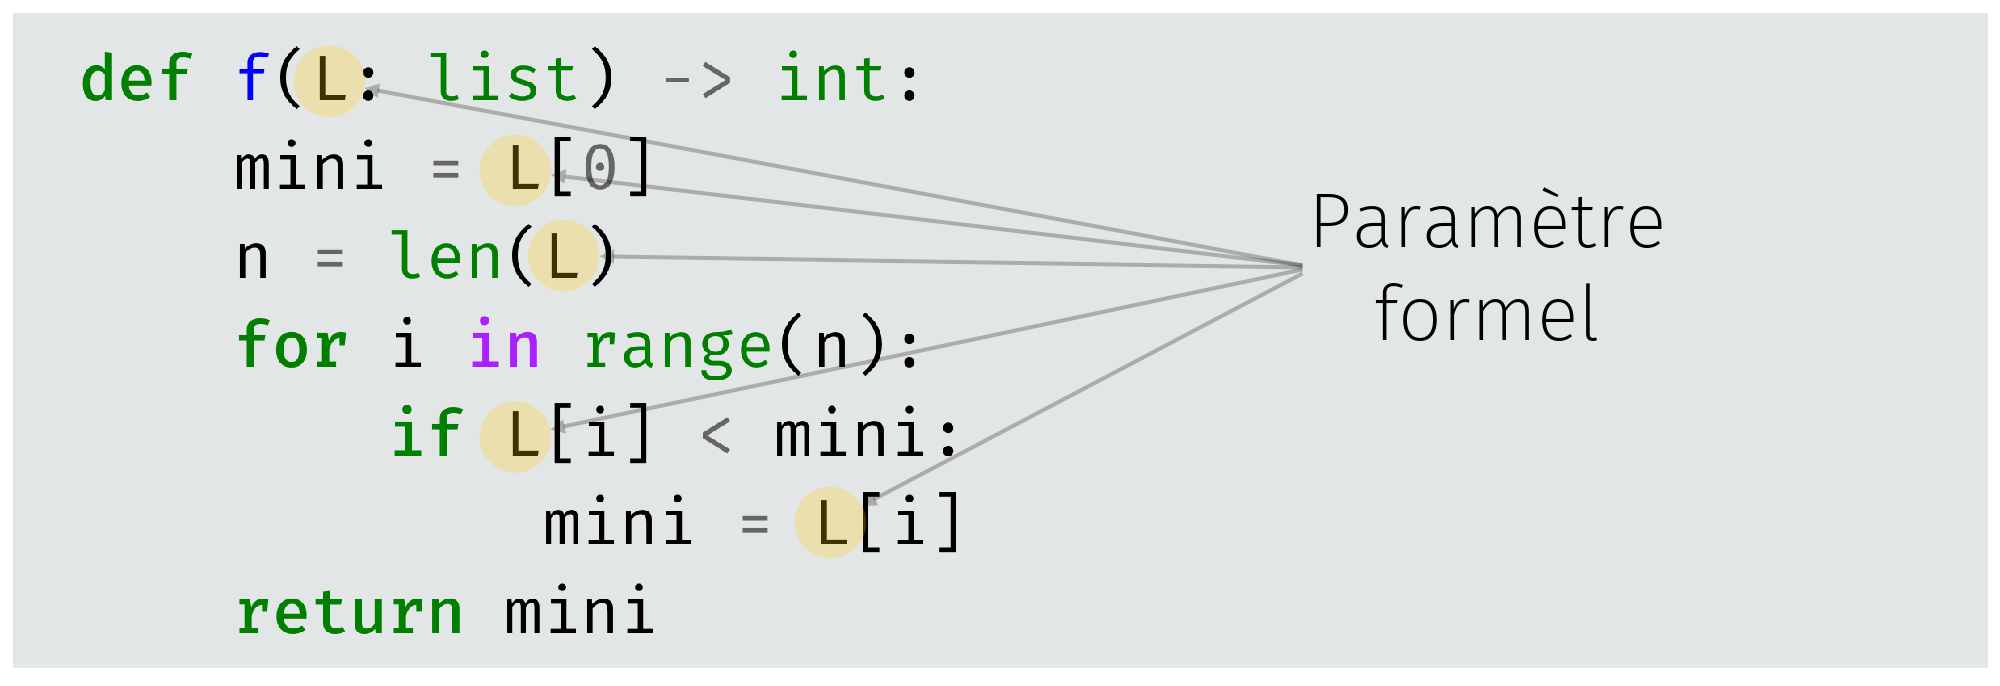
\includegraphics[width=10cm]{img/anat1}
\end{center}
Le paramètre d'entrée est \textit{formel} : \textit{le nom de cette variable n'existe qu'à l'intérieur de la fonction}.
Si ce nom de variable existe déjà à l'extérieur de la fonction, \textit{ce n'est pas la même variable}.\\
\begin{center}
    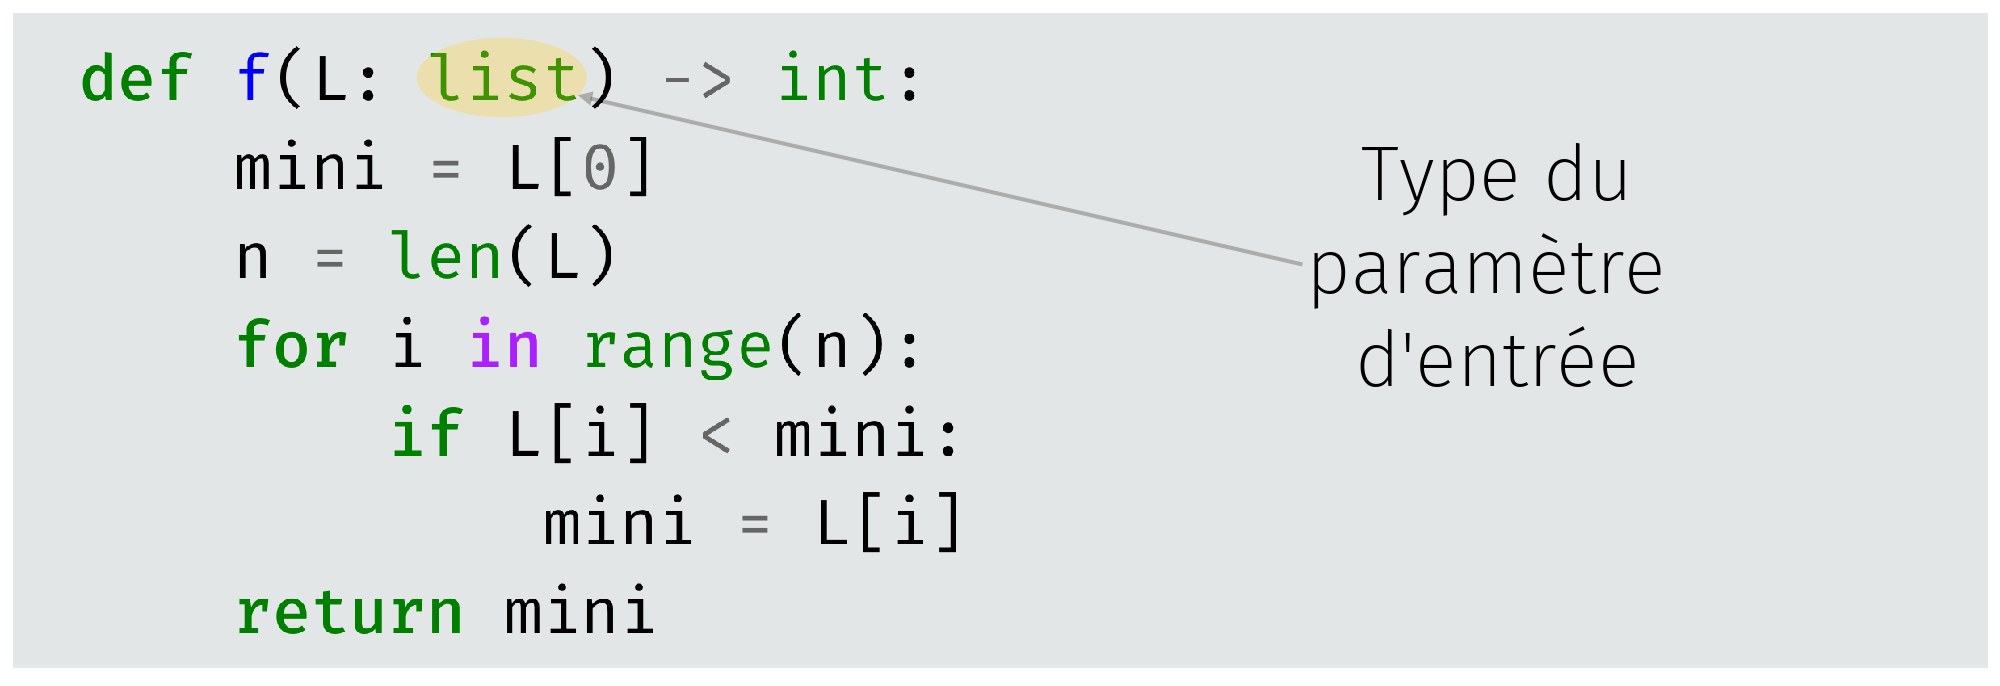
\includegraphics[width=10cm]{img/anat4}
\end{center}
Le type du paramètre d'entrée peut être spécifié. Ce n'est pas obligatoire mais très fortement recommandé pour \og garder les idées claires\fg{}.\\

\begin{center}
    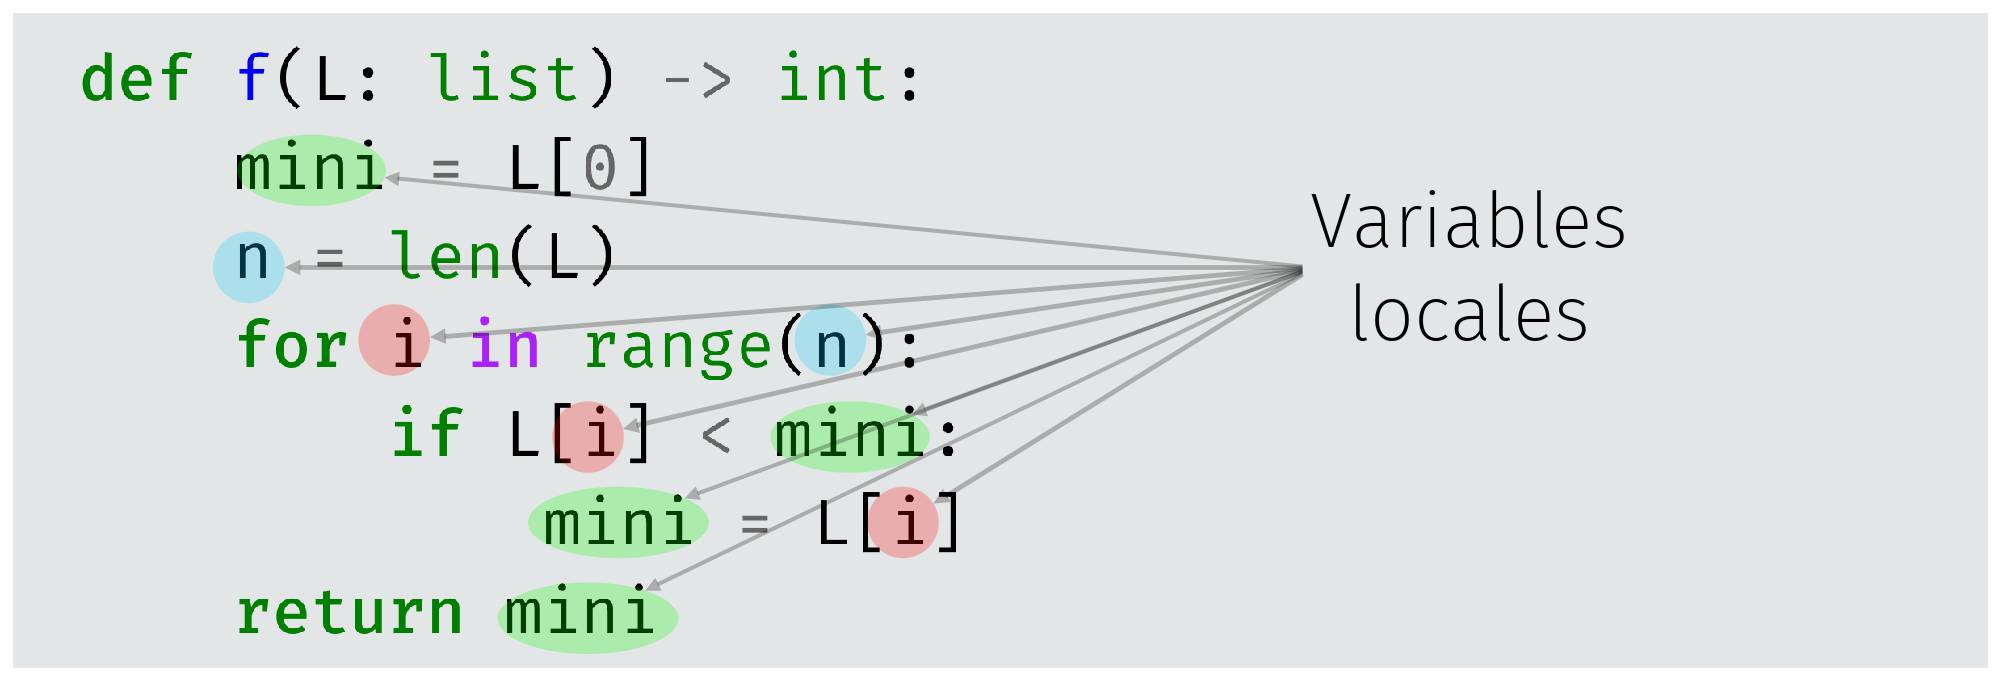
\includegraphics[width=10cm]{img/anat2}
\end{center}
Toutes les variables \textit{créées} dans une fonction n'existent \textit{que dans cette fonction}. Elles ne sont pas accessibles depuis l'extérieur de la fonction. On dit que ce sont des \textit{variables locales}.\\

\subsection{valeur de sortie}
\begin{center}
    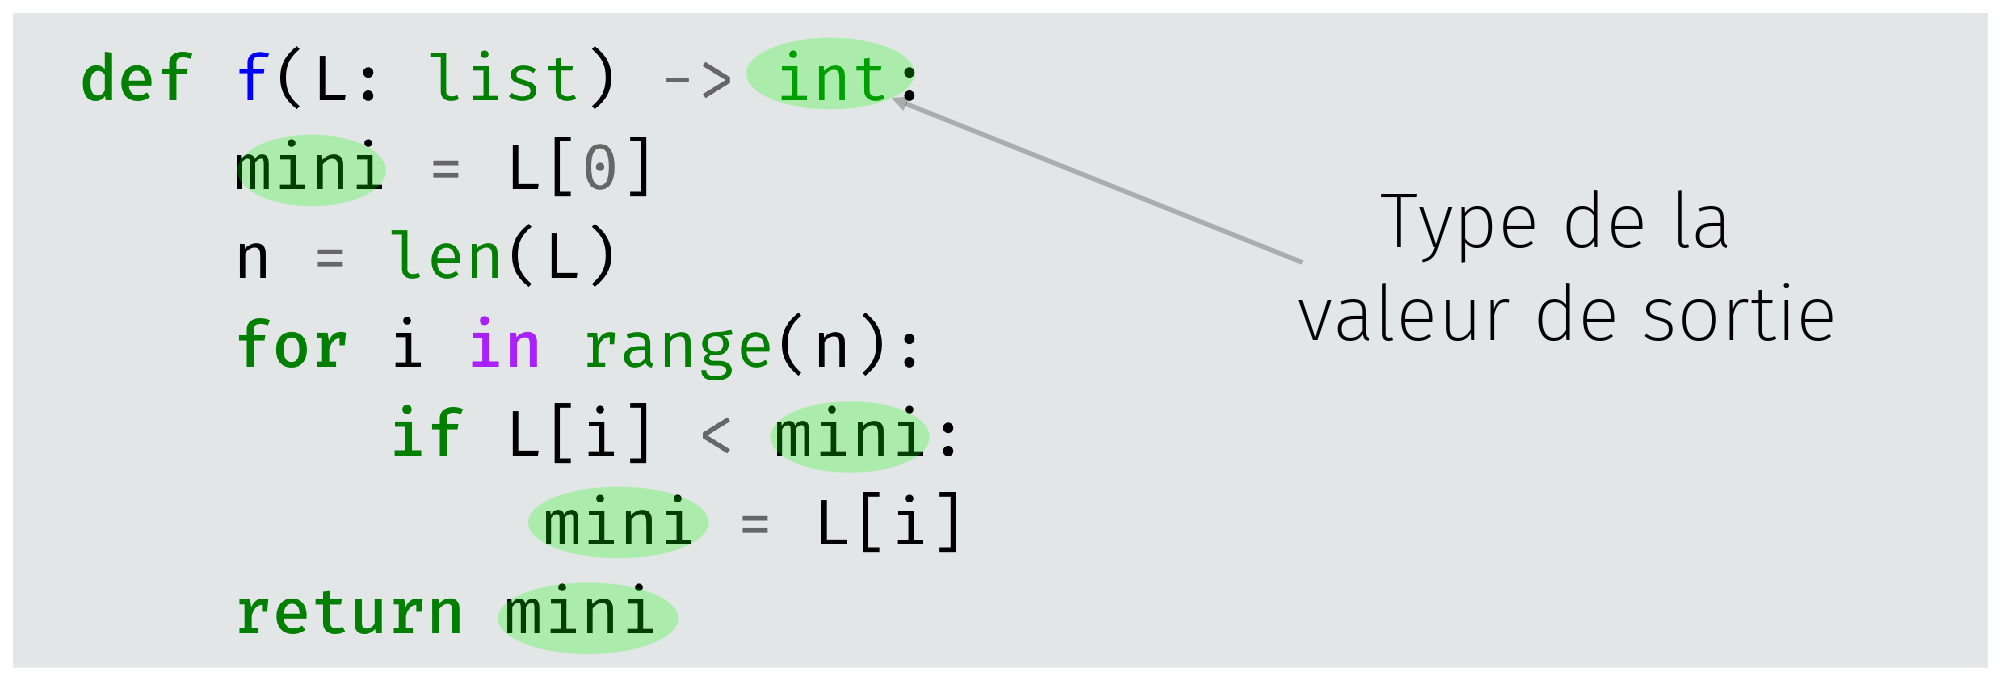
\includegraphics[width=10cm]{img/anat3}
\end{center}
Le type de la valeur de sortie peut être précisé, c'est également recommandé.

\section{En pratique}
\subsection{Des exemples}
 \begin{pyc}
\begin{minted}{python}
1   def f(x : float) -> float:
2       return x ** 2 + 3 * x + 2
3    
4   print(f(1)) # Affiche 6
\end{minted}
\end{pyc}
Le programme commence à la ligne 4 !\\
Les 2 premières lignes servent à définir la fonction \texttt{f}, elles ne sont exécutées que lorsqu'on évalue \texttt{f(1)}.\\



\begin{pyc}
\begin{minted}{python}
def f(x : float) -> float:
    return x ** 2 + 3 * x + 2
    
print(x) # Provoque une erreur
\end{minted}
\end{pyc}
L'erreur vient du fait que la variable \texttt{x} \textit{n'est pas définie}. Le \og \texttt{x} qu'on voit dans la fonction \texttt{f}\fg{} est un paramètre formel et n'existe que dans \texttt{f}.\\


\begin{pyc}
\begin{minted}{python}
def f(x : float) -> float:
    a = 2
    return x + a

print(a) # Provoque une erreur
    \end{minted}
\end{pyc}
L'erreur vient du fait que la variable \texttt{a} \textit{est locale} : elle n'est définie que durant l'exécution de \texttt{f}.\\

\begin{pyc}
\begin{minted}{python}
def f(x : float) -> float:
    a = 2
    return x + a

print(f(4)) # Affiche 6        
print(a) # Provoque une erreur
    \end{minted}
\end{pyc}
C'est encore la même erreur : une fois \texttt{f(4)} évaluée, \texttt{a} n'existe plus.\\

\begin{pyc}
\begin{minted}{python}
1   def f(x : float) -> float:
2       a = 2
3       return x + a
4
5   a = 3
6   print(f(4)) # Affiche 6
7   print(a) # Affiche 3 et pas 2
\end{minted}
\end{pyc}

La variable \texttt{a} définie dans la fonction \texttt{f} n'est pas la même que celle qui est définie à la ligne 5.\\
Celle définie à la ligne 2 est \textit{locale}.\\
La variable \texttt{a} de la ligne 5 est appelée \textit{globale}.\\



\begin{pyc}
\begin{minted}{python}
def f(x : float) -> float:
    return x + a
        
a = 3
print(f(4)) # Affiche 7
\end{minted}
\end{pyc}
\begin{aretenir}
Une fonction a le droit d'\textit{accéder en lecture} à une variable globale, mais n'a pas \textit{a priori} le droit d'en modifier la valeur.
\end{aretenir}

\subsection{À éviter autant que possible}



\begin{pyc}
\begin{minted}{python}
1   def f(x : float) -> float:
2       global a 
3       a = a + 1
4       return x + a
5        
6   a = 3
7   print(f(4)) # Affiche 8
8   print(a) # Affiche 4       
\end{minted}
\end{pyc}
À la ligne 2, on signale à Python que \texttt{f} a la droit de modifier la variable globale \texttt{a}.
C'est fortement déconseillé : sauf si on ne peut pas faire autrement, une fonction ne doit pas modifier les variables globales.